\chapter{Gegenereerde beschrijvingen}
\label{app:generalResults}
Deze bijlage bevat een aantal voorbeelden van zinnen gegenereerd door het gLSTM model met als gids LDA met 120 topics en generatie zonder normalisatie. We onderscheiden drie categorie\"en. E\'en voor quasi-perfecte beschrijvingen, \'e\'en voor beschrijvingen waarin het overgrote deel klopt maar bepaalde aspecten fout zijn en \'e\'en voor beschrijvingen die niets of weinig met de afbeelding te maken hebben.
	\begin{figure}
		\begin{subfigure}{.5\textwidth}
			\centering
			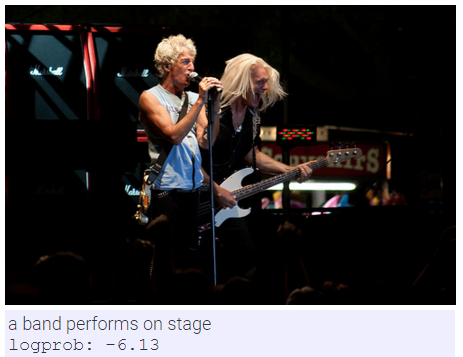
\includegraphics[width=.8\linewidth]{Images/Results/Perfect/band_performs}
			\label{fig:perfectresults1}
		\end{subfigure}%
		\begin{subfigure}{.5\textwidth}
			\centering
			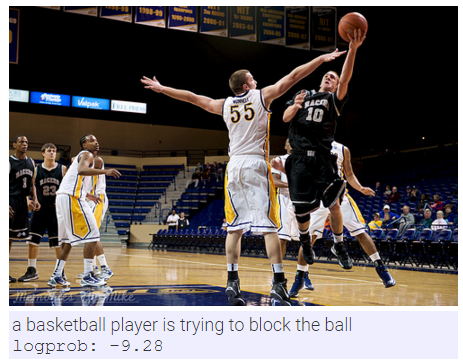
\includegraphics[width=.8\linewidth]{Images/Results/Perfect/blocking_the_ball}
			\label{fig:perfectresults2}
		\end{subfigure}\\
		\begin{subfigure}{.5\textwidth}
			\centering
			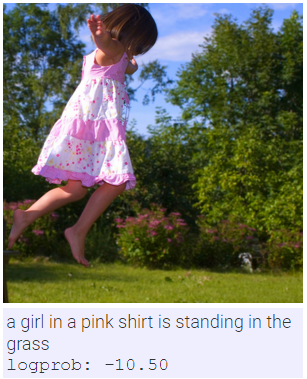
\includegraphics[width=.8\linewidth]{Images/Results/Perfect/girl}
			\label{fig:perfectresults3}
		\end{subfigure}%
		\begin{subfigure}{.5\textwidth}
			\centering
			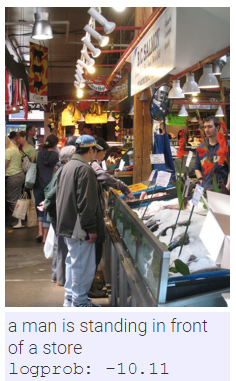
\includegraphics[width=.8\linewidth]{Images/Results/Perfect/main_in_front_of_store}
			\label{fig:perfectresults4}
		\end{subfigure}				
		
		\caption{Quasi-perfecte resultaten gegenereerd door gLSTM+LDA 120}
		\label{fig:perfectresults}
	\end{figure}
	
		\begin{figure}
			\begin{subfigure}{.5\textwidth}
				\centering
				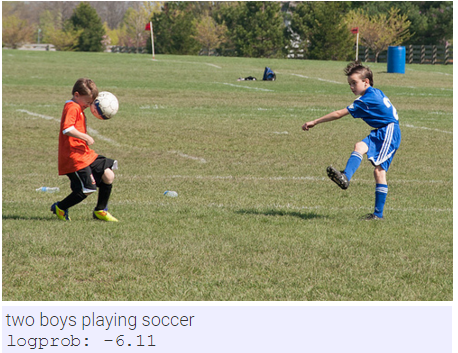
\includegraphics[width=.8\linewidth]{Images/Results/Perfect/playing_soccer}
				\label{fig:perfectresults5}
			\end{subfigure}%
			\begin{subfigure}{.5\textwidth}
				\centering
				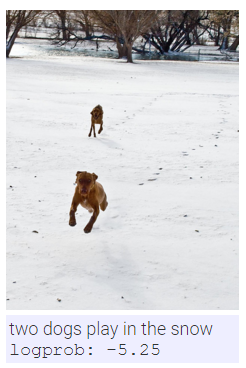
\includegraphics[width=.8\linewidth]{Images/Results/Perfect/two_dogs_in_snow}
				\label{fig:perfectresults6}
			\end{subfigure}
			\\
			\begin{subfigure}{.5\textwidth}
				\centering
				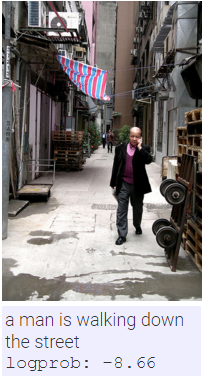
\includegraphics[width=.8\linewidth]{Images/Results/Perfect/walking_down_the_street}
				\label{fig:perfectresults7}
			\end{subfigure}%
			\begin{subfigure}{.5\textwidth}
				\centering
				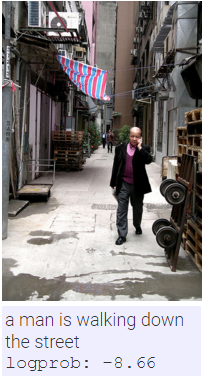
\includegraphics[width=.8\linewidth]{Images/Results/Perfect/walking_down_the_street}
				\label{fig:perfectresults8}
			\end{subfigure}	
			\caption{Quasi-perfecte resultaten gegenereerd door gLSTM+LDA 120 (vervolg)}
			\label{fig:perfectresults_2}
		\end{figure}
\todo[inline]{Nog ene vervangen}

% INTERMEDIATE

	\begin{figure}
		\begin{subfigure}{.5\textwidth}
			\centering
			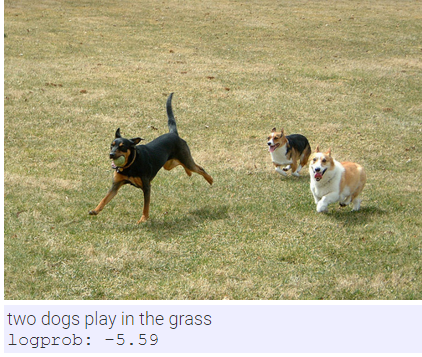
\includegraphics[width=.8\linewidth]{Images/Results/Intermediate/dogs_in_grass}
			\label{fig:intermediateresults1}
		\end{subfigure}%
		\begin{subfigure}{.5\textwidth}
			\centering
			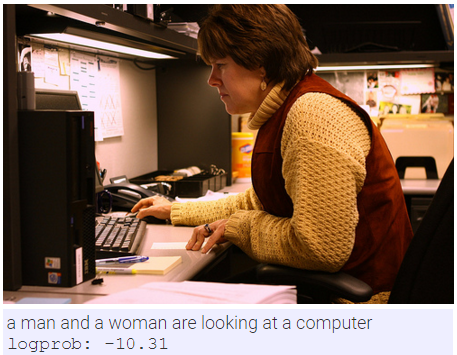
\includegraphics[width=.8\linewidth]{Images/Results/Intermediate/looing_at_computer}
			\label{fig:intermediateresults2}
		\end{subfigure}\\
		\begin{subfigure}{.5\textwidth}
			\centering
			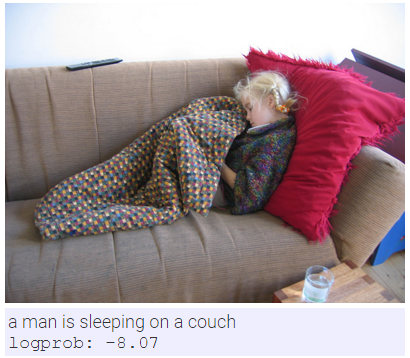
\includegraphics[width=.8\linewidth]{Images/Results/Intermediate/sleeping_couch}
			\label{fig:intermediateresults3}
		\end{subfigure}%
		\begin{subfigure}{.5\textwidth}
			\centering
			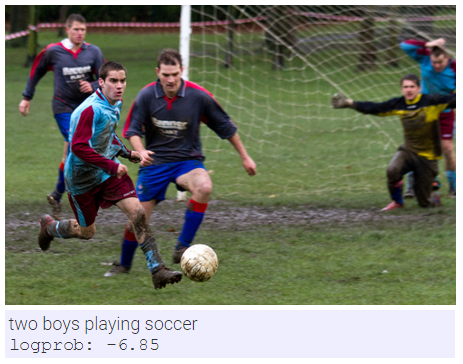
\includegraphics[width=.8\linewidth]{Images/Results/Intermediate/soccer}
			\label{fig:intermediateresults4}
		\end{subfigure}				\\
			\begin{subfigure}{.5\textwidth}
				\centering
				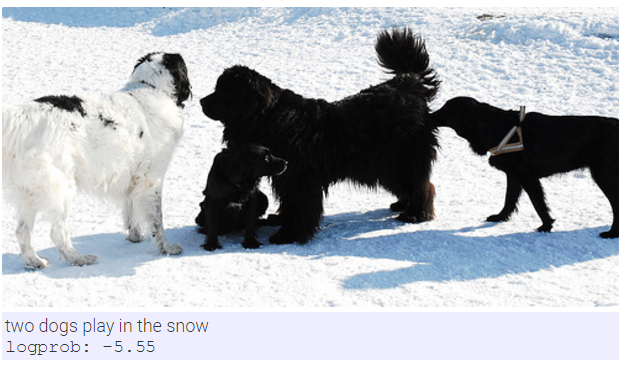
\includegraphics[width=.8\linewidth]{Images/Results/Intermediate/dogs_in_the_snow}
				\label{fig:intermediateresults5}
			\end{subfigure}%
			\begin{subfigure}{.5\textwidth}
				\centering
				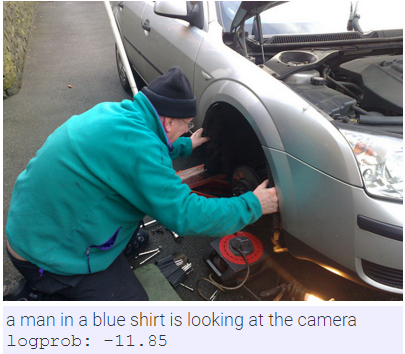
\includegraphics[width=.8\linewidth]{Images/Results/Intermediate/looking_at_camera}
				\label{fig:intermediateresults6}
			\end{subfigure}
		
		\caption{Resultaten gegenereerd door gLSTM+LDA 120 die kleine fouten vertonen}
		\label{fig:intermediateresult}
	\end{figure}

% BAD

	\begin{figure}
		\begin{subfigure}{.5\textwidth}
			\centering
			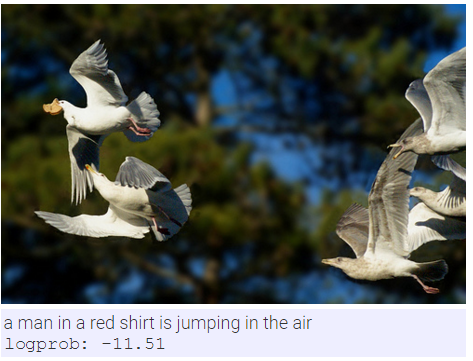
\includegraphics[width=.8\linewidth]{Images/Results/Bad/birds}
			\label{fig:badresults1}
		\end{subfigure}%
		\begin{subfigure}{.5\textwidth}
			\centering
			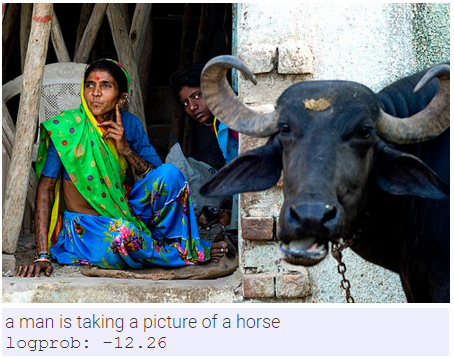
\includegraphics[width=.8\linewidth]{Images/Results/Bad/man_taking_picture_of_horse}
			\label{fig:badresults2}
		\end{subfigure}\\
		\begin{subfigure}{.5\textwidth}
			\centering
			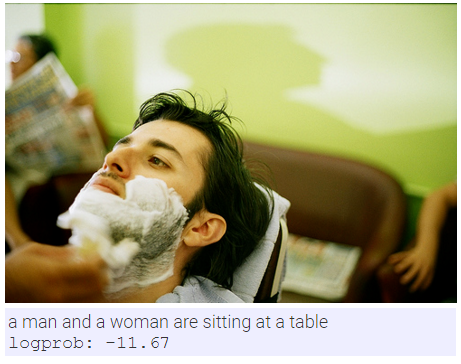
\includegraphics[width=.8\linewidth]{Images/Results/Bad/shaving}
			\label{fig:badresults3}
		\end{subfigure}%
		\begin{subfigure}{.5\textwidth}
			\centering
			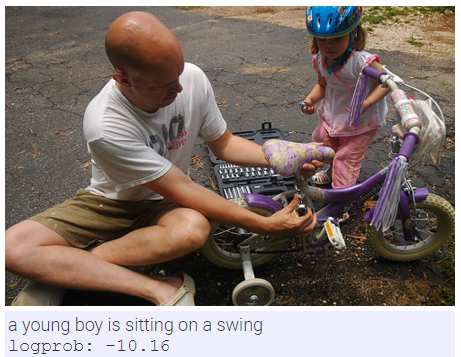
\includegraphics[width=.8\linewidth]{Images/Results/Bad/sitting_on_swing}
			\label{fig:badresults4}
		\end{subfigure}				\\
		\begin{subfigure}{.5\textwidth}
			\centering
			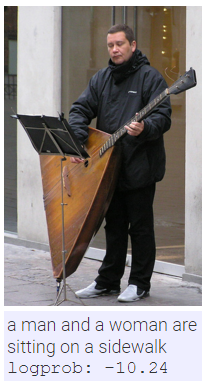
\includegraphics[width=.8\linewidth]{Images/Results/Bad/sitting_sidewalk}
			\label{fig:badresults5}
		\end{subfigure}%
		\begin{subfigure}{.5\textwidth}
			\centering
			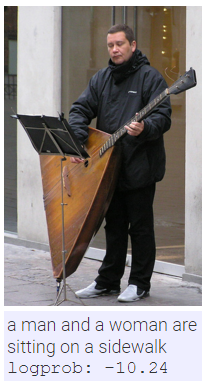
\includegraphics[width=.8\linewidth]{Images/Results/Bad/sitting_sidewalk}
			\label{fig:badresults6}
		\end{subfigure}
		
		\caption{Resultaten gegenereerd door gLSTM+LDA 120 die grote fouten vertonen}
		\label{fig:badresults}
	\end{figure}
	\todo[inline]{Ene extra}

